\documentclass[border=5pt]{standalone}
\usepackage{tikz}
\usetikzlibrary{positioning, arrows.meta, calc}
\usepackage{amsmath}
\usepackage{booktabs}

\newcommand{\Snbr}{S_{\text{nbr}}}

\begin{document}
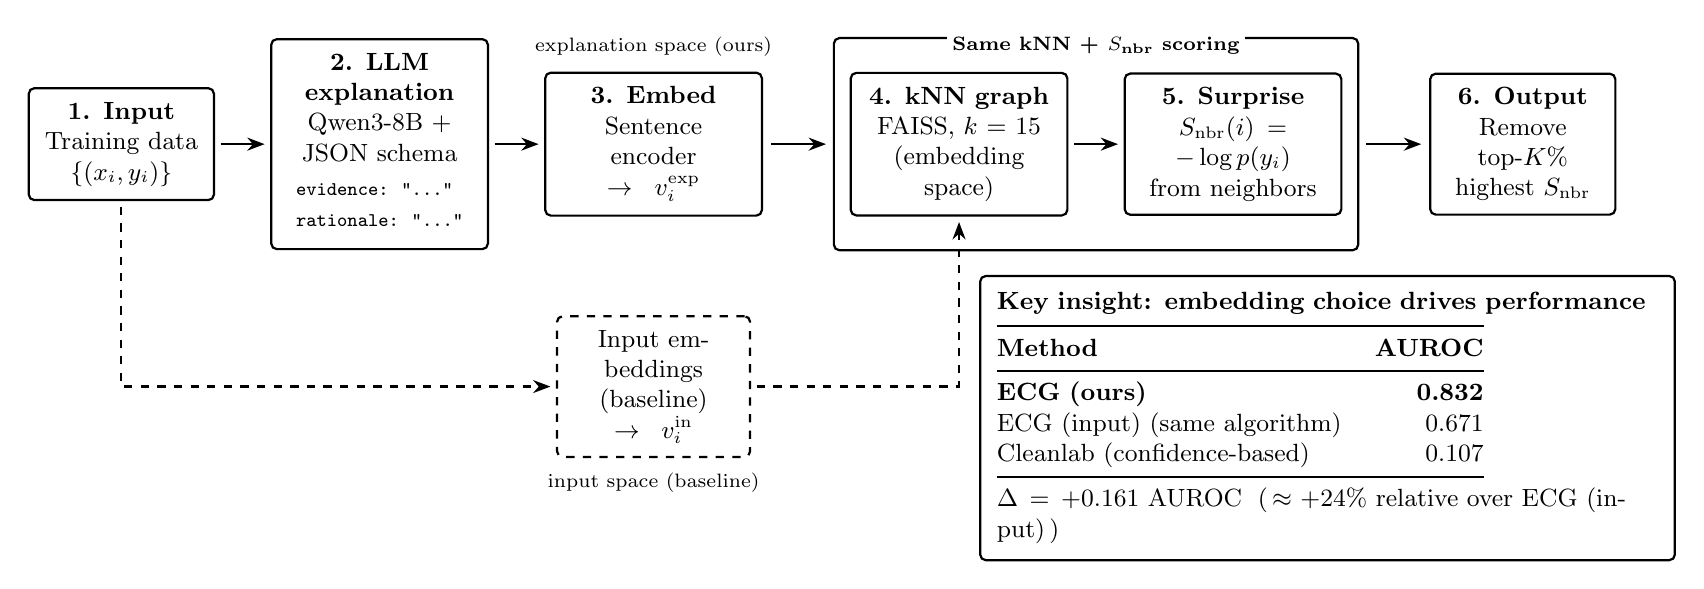
\begin{tikzpicture}[font=\small]

% ---------- Styles ----------
\tikzset{
  proc/.style={
    draw, rounded corners=2pt, thick,
    align=center, minimum height=1.35cm,
    inner sep=5pt
  },
  baseline/.style={proc, dashed},
  arrow/.style={
    -{Stealth[length=2.2mm]},
    thick, shorten >=2pt, shorten <=2pt
  },
  dashedarrow/.style={arrow, dashed},
  note/.style={
    draw, rounded corners=2pt, thick,
    align=left, inner sep=6pt
  }
}

% ---------- Main pipeline (ECG / ECG) ----------
\node[proc, text width=2.0cm] (data) {
  \textbf{1. Input}\\
  Training data\\
  $\{(x_i, y_i)\}$
};

\node[proc, text width=2.4cm, right=0.7cm of data] (llm) {
  \textbf{2. LLM explanation}\\
  Qwen3-8B + JSON schema\\[0.4em]
  \begin{tabular}{@{}l@{}}
    \scriptsize\ttfamily evidence: "..."\\
    \scriptsize\ttfamily rationale: "..."
  \end{tabular}
};

\node[proc, text width=2.4cm, right=0.7cm of llm] (embedexp) {
  \textbf{3. Embed}\\
  Sentence encoder\\
  $\rightarrow\ v_i^{\text{exp}}$
};

\node[proc, text width=2.4cm, right=1.1cm of embedexp] (knn) {
  \textbf{4. kNN graph}\\
  FAISS, $k=15$\\
  (embedding space)
};

\node[proc, text width=2.4cm, right=0.7cm of knn] (surprise) {
  \textbf{5. Surprise}\\
  $\Snbr(i)=-\log p(y_i)$\\
  from neighbors
};

\node[proc, text width=2.0cm, right=1.1cm of surprise] (out) {
  \textbf{6. Output}\\
  Remove top-$K\%$\\
  highest $\Snbr$
};

\draw[arrow] (data) -- (llm);
\draw[arrow] (llm) -- (embedexp);
\draw[arrow, shorten <=0.1cm, shorten >=0.3cm] (embedexp) -- (knn);
\draw[arrow] (knn) -- (surprise);
\draw[arrow, shorten <=0.3cm, shorten >=0.1cm] (surprise) -- (out);

% ---------- Baseline branch (ECG (input): same algorithm, different embedding) ----------
\node[baseline, text width=2.1cm, below=1.25cm of embedexp] (embedin) {
  Input embeddings\\
  (baseline)\\
  $\rightarrow\ v_i^{\text{in}}$
};

\draw[dashedarrow] (data.south) |- (embedin.west);
\draw[dashedarrow] (embedin.east) -| (knn.south);

% Small labels to make the contrast explicit
\node[font=\scriptsize, above=2pt of embedexp] {explanation space (ours)};
\node[font=\scriptsize, below=2pt of embedin] {input space (baseline)};

% ---------- Highlight: shared algorithm block ----------
% Highlight: shared algorithm block (aligned with llm's vertical bounds)
\coordinate (frame-tl) at ($(knn.west)+(-0.20,0)$);
\coordinate (frame-br) at ($(surprise.east)+(0.20,0)$);
\draw[thick, rounded corners=2pt]
  (frame-tl |- llm.north) rectangle
  (frame-br |- llm.south);

\node[font=\scriptsize\bfseries, anchor=south, fill=white, inner sep=2pt]
  at ($(knn.north)!0.5!(surprise.north)+(0,0.15)$)
  {Same kNN + $\Snbr$ scoring};

% ---------- Performance callout ----------
\node[note, text width=8.4cm, below=0.75cm of surprise, anchor=north, xshift=1.2cm] (perf) {
  \textbf{Key insight: embedding choice drives performance}\\[0.3em]
  \begin{tabular}{@{}l r@{}}
    \toprule
    \textbf{Method} & \textbf{AUROC} \\
    \midrule
    \textbf{ECG (ours)} & \textbf{0.832} \\
    ECG (input) (same algorithm) & 0.671 \\
    Cleanlab (confidence-based) & 0.107 \\
    \bottomrule
  \end{tabular}\\[0.3em]
  $\Delta=+0.161$ AUROC \;(\,$\approx$ +24\% relative over ECG (input)\,)
};

\end{tikzpicture}
\end{document}

